\subsection{UC-7}

\begin{figure}[H]
    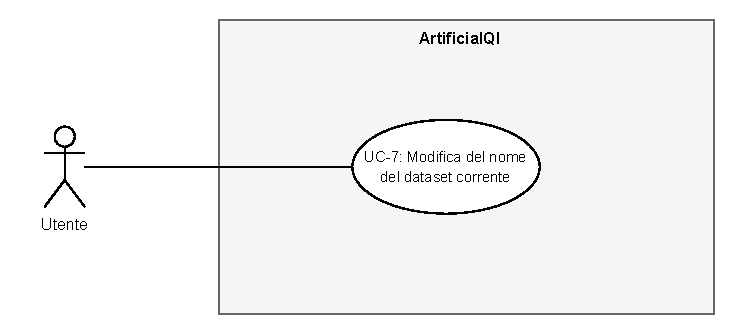
\includegraphics{Sezioni/UseCase/Immagini/UC-7.pdf}
    \caption{Diagramma UC-7.}
\end{figure}

\begin{usecase}{UC-7}{Modifica del nome del dataset corrente}
    
    \req{\hyperref[item:RU-1]{RU-1}} 

    \pre{
        \item Il sistema è attivo e funzionante
        \item Il dataset corrente non è vuoto 
    }

    \post{
        \item Il dataset corrente viene associato al nome indicato
    }
    
    \actor{Utente}

    \subactors{}

    \trigger{L'utente vuole modificare il nome del dataset corrente}
    
    \inc{}

    \base{}

    \scenario{
        \item L'utente richiede la modifica del nome del dataset corrente
        \item L'utente specifica il nuovo nome
        \item L'utente conferma la modifica 
        \item Il nuovo nome viene associato al dataset corrente
    }

    \subscenario{
        \item[2.1] \textbf{L'utente annulla l'operazione di modifica}
        \begin{itemize}
            \item [a.] \hyperref[subsec:UC-2]{UC-2}
        \end{itemize}
        \item[3.1] \textbf{Il nuovo nome del dataset è vuoto}
        \begin{itemize}
            \item [a.] \hyperref[subsec:UC-8]{UC-8}
        \end{itemize}
    }
\end{usecase}